\section*{Questões}
\paragraph{1.}

\subparagraph{a.}
Captura \emph{wireshark} na interface f1/1 de \textsf{R0}, do pedido de IP para interface \textsf{tap0} do \textsf{terminal 1}:

\begin{figure}[h]
\centering
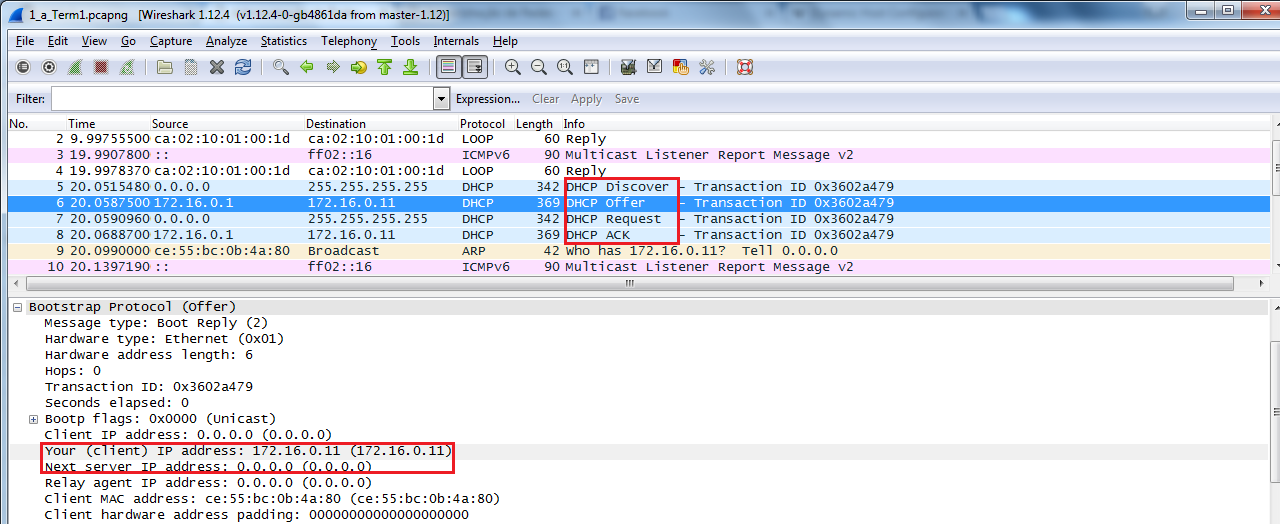
\includegraphics[width=1\textwidth, height=0.3\textheight]{1_a_Terminal1.png}
\label{fig:Term1 DHCP}
\caption{Terminal 1 obtém endereço IP por DHCP.}
\end{figure}

Captura \emph{wireshark} na interface f1/1 de \textsf{R0}, do pedido de IP para interface \textsf{eth0 } do \textsf{terminal 2}:

\begin{figure}[h]
\centering
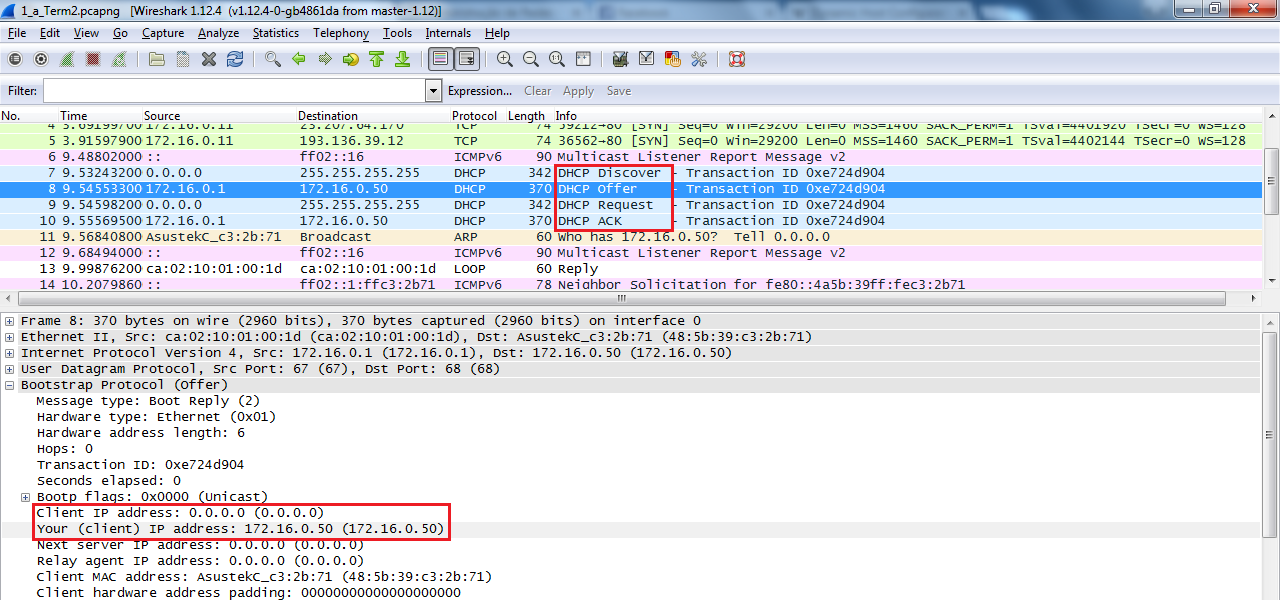
\includegraphics[width=1\textwidth, height=0.33\textheight]{1_a_Terminal2.png}
\label{fig:Term2 DHCP}
\caption{Terminal 2 obtém endereço IP por DHCP..}
\end{figure}


\subparagraph{b.}
Apenas a partir das mensagens capturadas é possível saber qual dos dois tem um endereço estático? Justifique.?????

\paragraph{2.}

\begin{verbatim}
Router#debug ip nat detailed
IP NAT detailed debugging is on
Router#
*May  4 15:48:31.783: NAT*: i: tcp (172.16.0.11, 48844) -> (162.125.64.1, 443) 
[878]
*May  4 15:48:31.783: NAT*: s=172.16.0.11->192.168.56.178, d=162.125.64.1 [878]
*May  4 15:48:31.939: NAT*: o: tcp (162.125.64.1, 443) -> (192.168.56.178, 48844)
 [49921]
*May  4 15:48:31.939: NAT*: s=162.125.64.1, d=192.168.56.178->172.16.0.11 [49921]
*May  4 15:48:31.939: NAT*: o: tcp (162.125.64.1, 443) -> (192.168.56.178, 48844)
[49922]
*May  4 15:48:31.939: NAT*: s=162.125.64.1, d=192.168.56.178->172.16.0.11 [49922]
*May  4 15:48:31.983: NAT*: i: tcp (172.16.0.11, 48844) -> (162.125.64.1, 443) 
[879]
*May  4 15:48:31.983: NAT*: s=172.16.0.11->192.168.56.178, d=162.125.64.1 [879]
*May  4 15:48:32.163: NAT*: o: tcp (162.125.64.1, 443) -> (192.168.56.178, 48844)
 [49923]
*May  4 15:48:32.163: NAT*: s=162.125.64.1, d=192.168.56.178->172.16.0.11 [49923]
*May  4 15:48:32.295: NAT*: i: tcp (172.16.0.11, 48844) -> (162.125.64.1, 443) 
[880]
*May  4 15:48:32.295: NAT*: s=172.16.0.11->192.168.56.178, d=162.125.64.1 [880]
*May  4 15:48:32.391: NAT*: o: tcp (162.125.64.1, 443) -> (192.168.56.178, 48844) 
[49924]
*May  4 15:48:32.391: NAT*: s=162.125.64.1, d=192.168.56.178->172.16.0.11 [49924]
*May  4 15:48:32.391: NAT*: o: tcp (162.125.64.1, 443) -> (192.168.56.178, 48844) 
[49925]
*May  4 15:48:32.391: NAT*: s=162.125.64.1, d=192.168.56.178->172.16.0.11 [49925]
*May  4 15:48:32.435: NAT*: i: tcp (172.16.0.11, 48844) -> (162.125.64.1, 443) 
[881]
*May  4 15:48:32.435: NAT*: s=172.16.0.11->192.168.56.178, d=162.125.64.1 [881]
*May  4 15:48:32.499: NAT*: o: tcp (162.125.64.1, 443) -> (192.168.56.178, 48844) 
[49926]
*May  4 15:48:32.499: NAT*: s=162.125.64.1, d=192.168.56.178->172.16.0.11 [49926]
*May  4 15:48:32.499: NAT*: o: tcp (162.125.64.1, 443) -> (192.168.56.178, 48844) 
[49927]
*May  4 15:48:32.499: NAT*: s=162.125.64.1, d=192.168.56.178->172.16.0.11 [49927]
*May  4 15:48:32.535: NAT*: i: tcp (172.16.0.11, 48844) -> (162.125.64.1, 443) 
[882]
*May  4 15:48:32.535: NAT*: s=172.16.0.11->192.168.56.178, d=162.125.64.1 [882]
*May  4 15:48:32.683: NAT*: o: tcp (162.125.64.1, 443) -> (192.168.56.178, 48844) 
[49928]
*May  4 15:48:32.683: NAT*: s=162.125.64.1, d=192.168.56.178->172.16.0.11 [49928]
*May  4 15:48:32.807: NAT*: i: tcp (172.16.0.11, 48280) -> (31.13.90.6, 443) 
[33593]
*May  4 15:48:32.807: NAT*: s=172.16.0.11->192.168.56.178, d=31.13.90.6 [33593]
*May  4 15:48:32.899: NAT*: o: tcp (31.13.90.6, 443) -> (192.168.56.178, 48280)
 [18010]
*May  4 15:48:32.899: NAT*: s=31.13.90.6, d=192.168.56.178->172.16.0.11 [18010]
*May  4 15:48:32.935: NAT*: i: tcp (172.16.0.11, 48280) -> (31.13.90.6, 443) 
[33594]
*May  4 15:48:32.935: NAT*: s=172.16.0.11->192.168.56.178, d=31.13.90.6 [33594]
*May  4 15:48:32.971: NAT*: o: tcp (162.125.64.1, 443) -> (192.168.56.178, 48844) 
[49929]
*May  4 15:48:32.971: NAT*: s=162.125.64.1, d=192.168.56.178->172.16.0.11 [49929]
*May  4 15:48:32.971: NAT*: o: tcp (162.125.64.1, 443) -> (192.168.56.178, 48844) 
[49930]
*May  4 15:48:32.971: NAT*: s=162.125.64.1, d=192.168.56.178->172.16.0.11 [49930]
*May  4 15:48:32.995: NAT*: i: tcp (172.16.0.11, 48844) -> (162.125.64.1, 443) 
[883]
*May  4 15:48:32.995: NAT*: s=172.16.0.11->192.168.56.178, d=162.125.64.1 [883]
*May  4 15:48:33.015: NAT: Allocated Port for 172.16.0.11 -> 192.168.56.178:
 wanted 39340 got 39340
*May  4 15:48:33.015: NAT*: i: tcp (172.16.0.11, 39340) -> (193.136.39.12, 80) 
[44778]
*May  4 15:48:33.015: NAT*: i: tcp (172.16.0.11, 39340) -> (193.136.39.12, 80)
[44778]
*May  4 15:48:33.019: NAT*: s=172.16.0.11->192.168.56.178, d=193.136.39.12 
[44778]
*May  4 15:48:33.051: NAT*: o: tcp (193.136.39.12, 80) -> (192.168.56.178, 39340)
 [0]
*May  4 15:48:33.051: NAT*: s=193.136.39.12, d=192.168.56.178->172.16.0.11 [0]
*May  4 15:48:33.059: NAT*: i: tcp (172.16.0.11, 39340) -> (193.136.39.12, 80)
 [44779]
*May  4 15:48:33.059: NAT*: s=172.16.0.11->192.168.56.178, d=193.136.39.12 
[44779]
*May  4 15:48:33.059: NAT*: i: tcp (172.16.0.11, 39340) -> (193.136.39.12, 80) 
[44780]
*May  4 15:48:33.059: NAT*: s=172.16.0.11->192.168.56.178, d=193.136.39.12
 [44780]

...
\end{verbatim}

Com base nas linhas de output de R0, explique o trabalho do NAT??????


\paragraph{3.}
comente a afirmação "Quando usamos NAT com tradução de portas, os fluxos de pacotes passam de connectionless para connection-oriented".??????


\paragraph{4.}

\subparagraph{a.}
\begin{verbatim}
[root@Labs5616 ar]# ssh 192.168.56.20
\end{verbatim}


\subparagraph{b.}
Identifique uma situação em que é necessário fazer port forwarding usando uma porta não-standard. ??????


\paragraph{5.}

\subparagraph{a.}

Justifique o insucesso deste procedimento. ????


\subparagraph{b.}
\begin{verbatim}
[root@Labs5616 Trab3]# iptables -t nat -A PREROUTING -p tcp -i enp0s7 
  -d 192.168.56.26 --dport 21 -j DNAT --to 10.0.0.22:21

[root@Labs5616 Trab3]# iptables-save
# Generated by iptables-save v1.4.21 on Wed May  4 17:54:11 2016
*nat
:PREROUTING ACCEPT [5:626]
:INPUT ACCEPT [1:328]
:OUTPUT ACCEPT [16:1194]
:POSTROUTING ACCEPT [3:234]
-A PREROUTING -d 192.168.56.26/32 -i enp0s7 -p tcp -m tcp --dport 21 
  -j DNAT --to-destination 10.0.0.22:21
-A POSTROUTING -o enp0s7 -j MASQUERADE
COMMIT
# Completed on Wed May  4 17:54:11 2016
# Generated by iptables-save v1.4.21 on Wed May  4 17:54:11 2016
*filter
:INPUT ACCEPT [21329:24200039]
:FORWARD ACCEPT [99770:70460139]
:OUTPUT ACCEPT [13750:876654]
COMMIT
# Completed on Wed May  4 17:54:11 2016
[root@Labs5616 Trab3]# 
\end{verbatim}


\subparagraph{c.}
Captura \emph{wireshark} na interface \textsf{enp0s7 - 192.168.56.26} do \textsf{Router Linux}:

\begin{figure}[h]
\centering
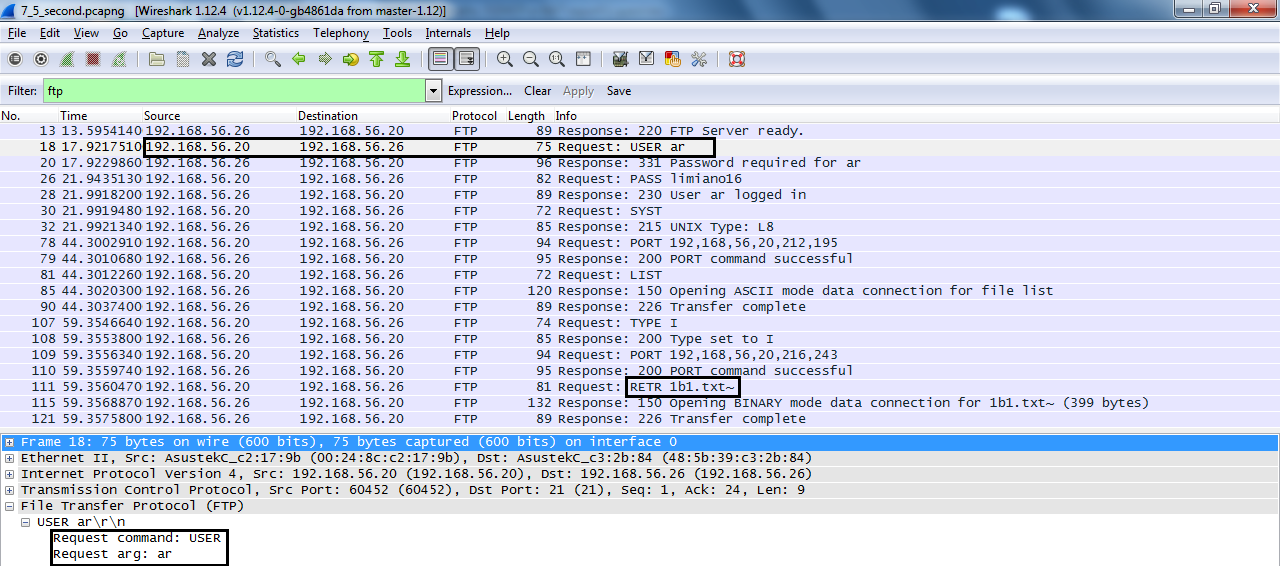
\includegraphics[width=1\textwidth, height=0.3\textheight]{5_b-enp0s7.png}
\label{fig:enp0s7}
\caption{Captura \emph{wireshark} na interface \textsf{192.168.56.26}.}
\end{figure}

Captura \emph{wireshark} na interface \textsf{enp1s6 - 10.0.0.1} do \textsf{Router Linux}:

\begin{figure}[h]
\centering
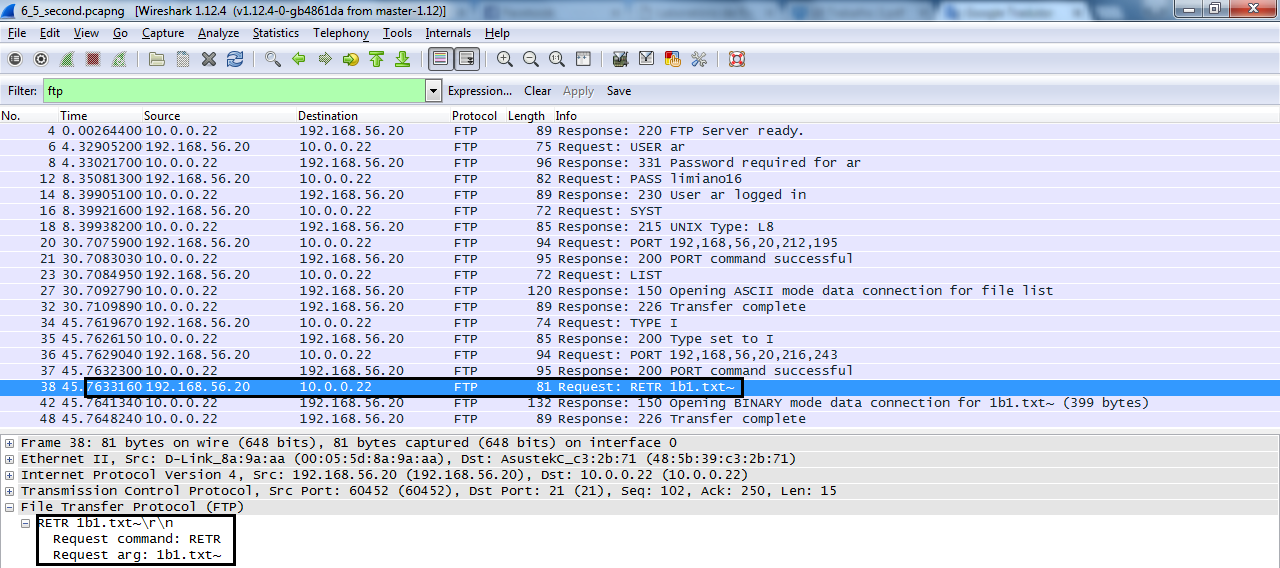
\includegraphics[width=1\textwidth, height=0.3\textheight]{5_b-enp1s6.png}
\label{fig:enp1s6}
\caption{Captura \emph{wireshark} na interface \textsf{10.0.0.1}.}
\end{figure}

comente os resultados?????


\subparagraph{d.}


\subparagraph{e.}

